\chapter{Implementation}\label{chap:implementation}
\begin{overview}

\end{overview}

\section{Segmentation}\label{sec:imp:segmentation}
\subsection{The Segmentation module}
The techniques described in section \ref{chap:lit:segmentation} were all implemented in a Python module called \modulename{Python}{segmentation}.

\subsection{Multi-objective fitting}
% TODO: Replace the reference to raquel with a cross-reference to the optimization chapter
As an example of the results obtainable using multi-objective optimisation, the MOPSO-CD algorithm discussed in section~\ref{sec:mopso} was used to fit a first-order response prototype to input signals.

A problem description based on a prototypical first order response was used in this study. Figure~\ref{fig:definition} shows the prototype function.
\begin{figure}[htbp]
  \centering
  \setlength{\unitlength}{1.8em}
  \begin{picture}(10,10) 
    \thicklines
    % axis
    \put(1,1){\vector(1,0){8}}
    
    \put(5,0){$t$}
    \put(1,1){\vector(0,1){8}}
    \put(0,7){$y_p$}
    % curve
    \qbezier(2,2)(4,8)(8,8)
    \put(2,2){\circle*{0.2}}
    \put(2,0){$t_{i-1}$}
    \put(0,2){$y_{i-1}$}

    \put(8,8){\circle*{0.2}} 
    \put(8,0){$t_i$}
    \put(0,8){$y_i$}

    \put(3,2){$\Delta t$}
    \put(3,1.8){\vector(-1,0){1}}
    \put(3,1.8){\vector(+1,0){2}}

    \put(6,1.7){$\Delta t_i$}
    \put(6,1.5){\vector(-1,0){4}}
    \put(6,1.5){\vector(+1,0){2}}
    
    \thinlines
    \put(2,2){\line(-1,0){1}}
    \put(2,2){\line(0,-1){1}}
    \put(8,8){\line(-1,0){7}}
    \put(8,8){\line(0,-1){7}}
    \put(5,7){\line(-1,0){4}}
    \put(5,7){\line(0,-1){6}}

  \end{picture}
  \caption{First order response prototype definition.  $\Delta t$ and $\Delta t_i$ are the times of the interpolation time and end point time relative to the prototype start.}
  \label{fig:definition}
\end{figure}

Our goal is to find a sequence of prototypes that fits the sequence of events.  
We wish to fit the entire data set, so the first and last times are to coincide with the first and last times in the data set.
Therefore, given that we are fitting $N$ prototypes, we seek to find $N-1$ transition times and $N$ parameter value sets.

A few key decisions ease optimisation.  
Firstly, a linear term  added to the exponential response ensures that the prototype interpolates through the initial $(x_{i-1}, y_{i-1})$ and final $(x_{i}, y_{i})$ points.  
This does add any parameters to the description.  
The predicted value for the prototype at a given time $t$ is shown in equation~\ref{eq:prototype}:
\begin{equation}
  \label{eq:prototype}
  y_p = y_{i-1} + y_i \left (1 - \underbrace{e^{\Delta
        t/\tau_i}}_{\textrm{exponential}} + \underbrace{\frac{\Delta
        t}{\Delta t_i}e^{\Delta t_i/\tau_i}}_{\textrm{linear}} \right)
\end{equation}

Secondly, the optimisation parameters were chosen to reduce coupling in the problem parameters by using absolute times for each starting point and constraining these times to be sequential rather than time differences constrained to be positive.  
This reduced the effect of any one starting point on the error produced by the remaining fit functions.

\subsection{Objective functions}
Two objectives were defined: the RMS error of the fit over all the prototypes and the ``complexity'' of the fit, which was calculated as 
\begin{equation}
  c = \sum_i^{N} \frac{1}{\tau_i}.
\end{equation}

This complexity measure works due to the addition of the linear correction term, which dominates for large $\tau$, meaning that as $\tau$ increases, one sees more of the linear behaviour and less of the exponential.  
Therefore, larger $c$ corresponds to greater curvature of the fitting prototypes.

\subsection{Prototype to event mapping}
Each sequence of prototypes identified was mapped back to a sequence of event types by using the following heuristics:
\begin{itemize}
\item If the difference between the start and end values is less   than a cut-off value $\epsilon_c$, the prototype is taken to   represent a constant event.
\item If the time constant is larger than a cut-off time constant   $\tau_c$, it is taken as a ramp. 
\item If neither of these holds, the prototype is a first order response.
\end{itemize}

The values of $\epsilon_c$ and $\tau_c$ are problem-dependant and should be chosen to represent an insignificant change in $y$ and a large time constant (in the chosen time units) respectively.

\section{Model library}
\subsection{Stream type}
A key element in the development of a Modelica chemical engineering simulation library is the encoding of the stream data in a stream type.  

%NOTE: Design only - replace by what was actually implemented - this probably
% needs to be in a separate file.

Intensive properties:
\begin{itemize}
  \item Pressure
  \item Temperature
\end{itemize}

Exensive properties:
\begin{itemize}
  \item Component mass flow rates (compositions come from flowrates)
\end{itemize}

To start building the simulation, the components have to be chosen and the initialiser has to be run.  
This creates the stream types that can be used in the rest of the unit operations.  
Simulation will fail if the component list is changed without re-running the initialiser.	

\subsection{Connector philiosophy}
%NOTE: This is rambling, but I'm getting my thoughts on paper
Blocks in Modelica are connected by connector types.  
The variables in the connectors can connect as ``flow-type'' variables or ``potential-type'' variables.  
The difference is in how the sign of equality is handled when the model is constructed.  
Flow-type variables are connected with a negative sign (so that flow out of one block is equal to the flow into another, but in the opposite direction), while potential-type variables are simply set equal to one another (this works well for things like pressure).

It was decided to bundle the extensive properties of the stream and the intensive properties of the stream seperately.

\section{CORBA support}
There are two popular patterns for the use of CAPE-OPEN when developing custom simulation codes.  
The first is to make use of the Unit Operation support to embed a unit operation into an existing flowsheeting package, which then handles the simulation calculations. 
The second is to use a stand-alone modelling environment, but to interface with various packages for information like thermodynamic properties, equilibrium and/reaction kinetics.  
It was decided to abstract the property and equilibrium calculations into a class (SimulationStream) which is specified as a connector type for the column components.  
The SimulationStream objects that are instantiated when the components are simulated communicate with a host using the ICapeThermoPropertyPackage methods CalcProp and CalcEquilibrium.  
The interfacing is done using CORBA.  
Mico CORBA was used on the client (Linux) machine, accessed using the support for external C routines in OpenModelica.  
On the host (Windows) machine, the Unisim CORBA Server was used to interface with Unisim.

Figure~\ref{fig:dataflow} shows the data flow conceptually.
\begin{figure}[htbp]
  \centering
  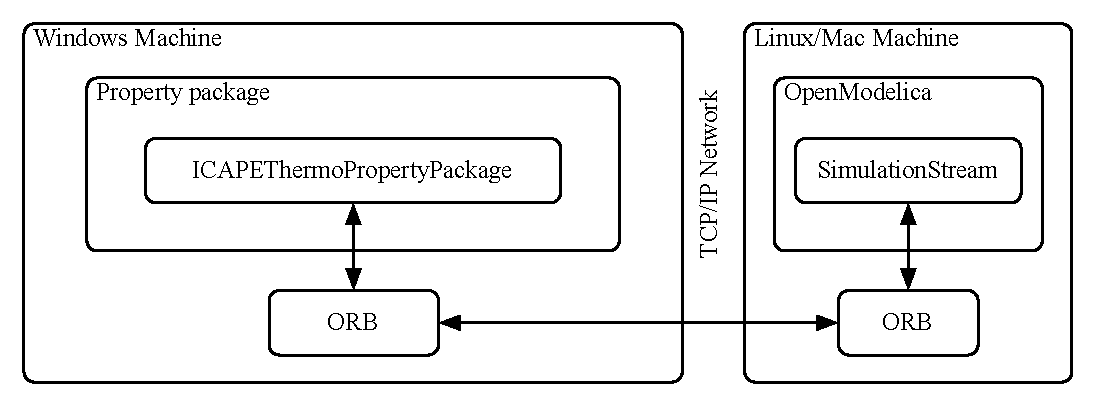
\includegraphics[width=0.9\textwidth]{dataflow}
  \caption{Simulation data flow for multiple computers}
  \label{fig:dataflow}
\end{figure}

It should be noted that, although this implementation has used CORBA due to the lack of support of COM on the Linux platform, CO-LaN supplies a COM-to-CORBA bridge as part of the CAPE-OPEN effort, so using CORBA is not a significant problem.

\section{Column model}
\label{sec:column-model} 
The distillation column modelled is a lab-scale glass distillation column fitted with a water-cooled total condenser and a steam thermosyphon boiler.  
It separates a mixture of ethanol and water.

The Modelica components developed for modelling the distillation column are shown schematically in Figure~\ref{fig:components}
\begin{figure}[htbp]
  \centering
  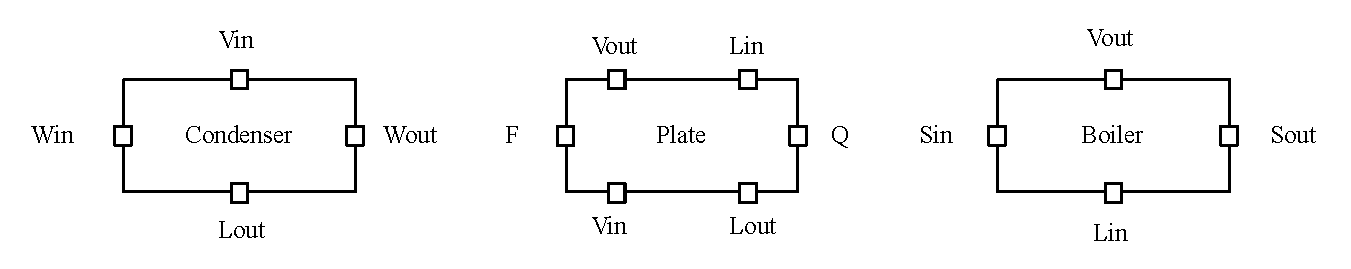
\includegraphics[width=\textwidth]{components}
  \caption{Distillation column components}
  \label{fig:components}
\end{figure}

A single generic plate model was developed that allows for a material and energy stream (both of which could be incoming or outgoing, labelled F and Q in the diagram) in addition to the normal vapour and liquid arrangement (two vapour streams and two liquid streams).  
This allows multiple feed columns to be modelled easily, even when the feeds are intermittend during the simulation.  
It also allows for energy losses or additions.  
The physical column that was modelled exhibits significant heat losses.

The plate model assumes negligible vapour dynamics, with per-component hold-up on the liquid side.  
The pressure drop between the input and output vapour streams is estimated using the height of liquid on the plate.  
The Wilson thermodynamic model was used as it accurately describes the ethanol-water equilibrium. 

The material streams these components are specified as SimulationStreams, allowing the material properties and equilibrium to be calculated by the external thermo host.


% Local Variables:
% TeX-master: "thesis"
% End:
